%This is a template for the University of Helsinki. If you have questions regarding the template please be in contact with uhbrand@helsinki.fi


\documentclass[11pt, aspectratio=169]{beamer}
  % papersize={16cm,9cm},

\mode<presentation>{}

%%%%%%%%%%%%%%%%%%%%%%%%%%%%%%
% Fill in the following information: AUTHOR, TITLE, DATE

\author[Roman Kyrychenko]{Roman Kyrychenko}
\title[Analysis of Reproducibility]{Analysis of the Reproducibility of the Study}
\date{date}%{\today}
\institute{Faculty of Social Sciences, University of Helsinki}
%%%%%%%%%%%%%%%%%%%%%%%%%%%%%%
% load packages
% add packages if needed

\usepackage[T1]{fontenc}
\usepackage[english]{babel}
\usepackage{amsmath,amsfonts,amssymb,amsthm}
\usepackage{color}
\usepackage[tracking=smallcaps, letterspace=-55]{microtype} % package for font spacing

\usepackage{transparent} % for setting opacity of pictures
\usepackage{pifont} % for checkmark (\ding{51}) and cross (\ding{55})
\usepackage{booktabs,array} % for tables
\usepackage{graphicx} % for figures
%\graphicspath{} % to set the path of figures

%%%%%%%%%%%%%%%%%%%%%%%%%%%%%%
% set beamer colors

\definecolor{hyblue}{RGB}{0,155,255}
\setbeamercolor{alerted text}{fg=hyblue}
\setbeamercolor{structure}{fg=hyblue}
\setbeamercolor{item}{fg=black}

%\setbeamertemplate{itemize item}{\bullet}

%%%%%%%%%%%%%%%%%%%%%%%%%%%%%%
% set font (helvetica plays the role of Arial)
\usepackage{helvet}
\renewcommand{\familydefault}{\sfdefault}

%%%%%%%%%%%%%%%%%%%%%%%%%%%%%%
% set frametitle

\setbeamercolor{frametitle}{fg=black}%{fg=hyblue}
\setbeamerfont{frametitle}{series=\bfseries, size=\huge}
\setbeamertemplate{frametitle}[default][left,leftskip=3.5cm] % left shift of frame title
\addtobeamertemplate{frametitle}{\vspace{0.5cm}}{\vspace{1cm}} % spacing above and below frame title

%%%%%%%%%%%%%%%%%%%%%%%%%%%%%%
% transparent box behind the title

\usepackage[many]{tcolorbox}
\usepackage{textcomp}
\usepackage{hyperref}

\newtcolorbox{titlebox}[1][]{
    width=\columnwidth,
    boxsep=0cm,
    toprule=1pt,
    leftrule=1pt,
    bottomrule=1pt,
    rightrule=1pt,
    colback=black,
    fontupper=\huge,
    breakable,
    nobeforeafter,
    enhanced,
    opacityframe=0.0,
    opacityback=0.7
}

%%%%%%%%%%%%%%%%%%%%%%%%%%%%%%
% set footline and headline
\beamertemplatenavigationsymbolsempty
\setbeamertemplate{headline}{ }
\setbeamertemplate{footline}{%
	 \usebeamercolor[fg]{page number in head/foot}%
	 \usebeamerfont{page number in head/foot}%
	\hspace{0.5cm}
	
\includegraphics[width=2.5cm]{images/HY__LC05_txt__L_3L_B3____BW_cropped}
	\hfill
	\insertshorttitle\ /\ \insertshortauthor	\hfill
	\today	\hspace{0.5cm}
	\insertframenumber\,/\,\inserttotalframenumber \hspace{0.5cm} \vskip2pt%
}

%%%%%%%%%%%%%%%%%%%%%%%%%%%%%%
% Other style settings
\setbeamertemplate{itemize items}[circle] % makes the bullets in lists circles

\begin{document}

\section{titleslides}

% Title slide with HY picture
{
\usebackgroundtemplate{
\setlength{\unitlength}{1cm}
\begin{picture}(16,9)

    % ON THE FOUR LINES BELOW, CHOOSE THE PICTURE RELATED TO YOUR CAMPUS BY HAVING '%' BEFORE THE ONES YOU DO NOT WISH TO USE AND REMOVING IT FROM THE ONE YOU DO WISH TO USE

    %\put(0.3,0.8){ 	\includegraphics[width=15cm,height=7.8cm]{original/Keskusta-hero.jpg} }
    %\put(0.3,0.8){ 	\includegraphics[width=15cm,height=7.8cm]{original/Viikki-hero.jpg} }
    \put(0.3,0.8){ 	
\includegraphics[width=15cm,height=7.8cm]{images/cover} }
    %\put(0.3,0.8){ 	\includegraphics[width=15cm,height=7.8cm]{original/Meilahti-hero.jpg} }

    % DO NOT TOUCH THIS ONE. IT PUTS THE LOGO IN ITS PLACE
    %\put(-0.5,5.4){ \includegraphics[width=5cm]{images/HY__LD01_LogoFP_EN_B3__NEGA (1)} }
\end{picture}
}
\setbeamertemplate{headline}{ }%
\begin{frame}{}
\vspace{5cm} % <-- ADJUST THIS TO MOVE THE TITLE UP OR DOWN IF NEEDED. SMALLER NUMBER TO MOVE IT UP, LARGER NUMBER TO MOVE DOWN
\begin{titlebox}[]
    \begin{center}
    {\bf \color{white} \MakeUppercase{\inserttitle} } \\
    {\large \color{white} \insertauthor}
    \end{center}
\end{titlebox}
\end{frame}
}



%% Title page without picture
%{
%\usebackgroundtemplate{
%\setlength{\unitlength}{1cm}
%\begin{picture}(16,9)
%	% BELOW YOU CAN CHANGE THE COLOR OF UNI LOGO ON THE TITLE PAGE IF YOU WISH. REMEMBER TO ALSO CHANGE IT ON THE CONTENT SLIDES FURTHER BELOW
%
%    \put(-0.1,5){ 
\includegraphics[width=4cm]{images/HY__LA01_Flame_____B3____BW} } % BLACK UNI LOGO
%    %\put(-0.1,5){ \includegraphics[width=4cm]{HY__LO01_matemF____B3___RGB.jpg} } % ORANGE UNI LOGO
%\end{picture}
%\setlength{\unitlength}{1pt}
%}
%\setbeamertemplate{headline}{ }%
%\begin{frame}[noframenumbering]{}
%\vspace{2.5cm}
%\begin{center}
%\huge
%\textcolor{hyblue}{ \bf
%\MakeUppercase{\inserttitle}
%} \\
%{\large
%\insertauthor}
%\end{center}
%\end{frame}
%}
%%

%%%%%%%%%%%%%%%%%%%%%%%%%%%%%%
%% Main text

%% set HY Logo on the upper-left corner:
\usebackgroundtemplate{
\setlength{\unitlength}{1cm}
\begin{picture}(16,2.5)
    % BELOW YOU CAN CHANGE THE COLOR OF UNI LOGO ON THE CONTENT PAGES IF YOU WISH. REMEMBER TO ALSO CHANGE IT ON THE TITLE SLIDE ABOVE

    \put(0.1,0){ 
\includegraphics[width=2.5cm]{images/HY__LA01_Flame_____B3____BW}\hfill } % BLACK UNI LOGO
    %\put(0.1,0){ \includegraphics[width=2.5cm]{HY__LO01_matemF____B3___RGB.jpg}\hfill } % ORANGE UNI LOGO
\end{picture}
\setlength{\unitlength}{1pt}
}
%%

%%%%%%%%%%%%%%%%%%%%%%%%%%%%%%
%% Modify text below


\begin{frame}{\MakeUppercase{What authors did}}

\begin{columns}[c]
    \begin{column}{.5\textwidth}
        \uncover<1->{
        \begin{itemize}
            \item Stack model: random forest + Feed forward neural network
        \end{itemize}
        }
        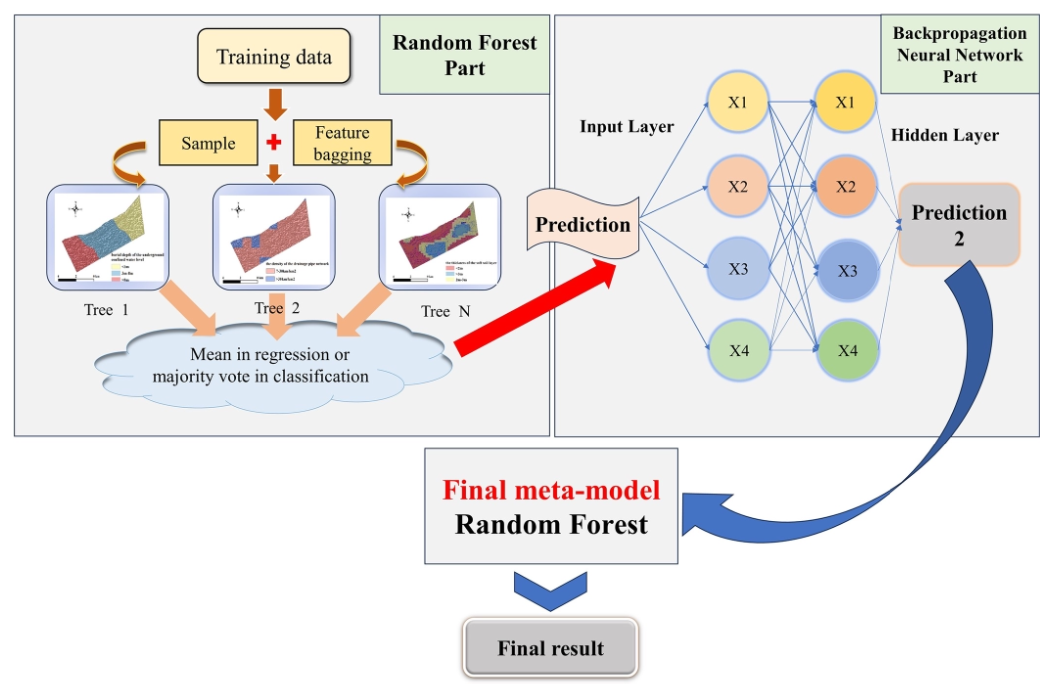
\includegraphics[width=7cm,height=4.5cm]{images/algo}
    \end{column}
    \begin{column}{.5\textwidth}
        \uncover<1->{
        \begin{itemize}
            \item ChatGPT-based decision on weights and its comparison to expert weights
        \end{itemize}
        }
        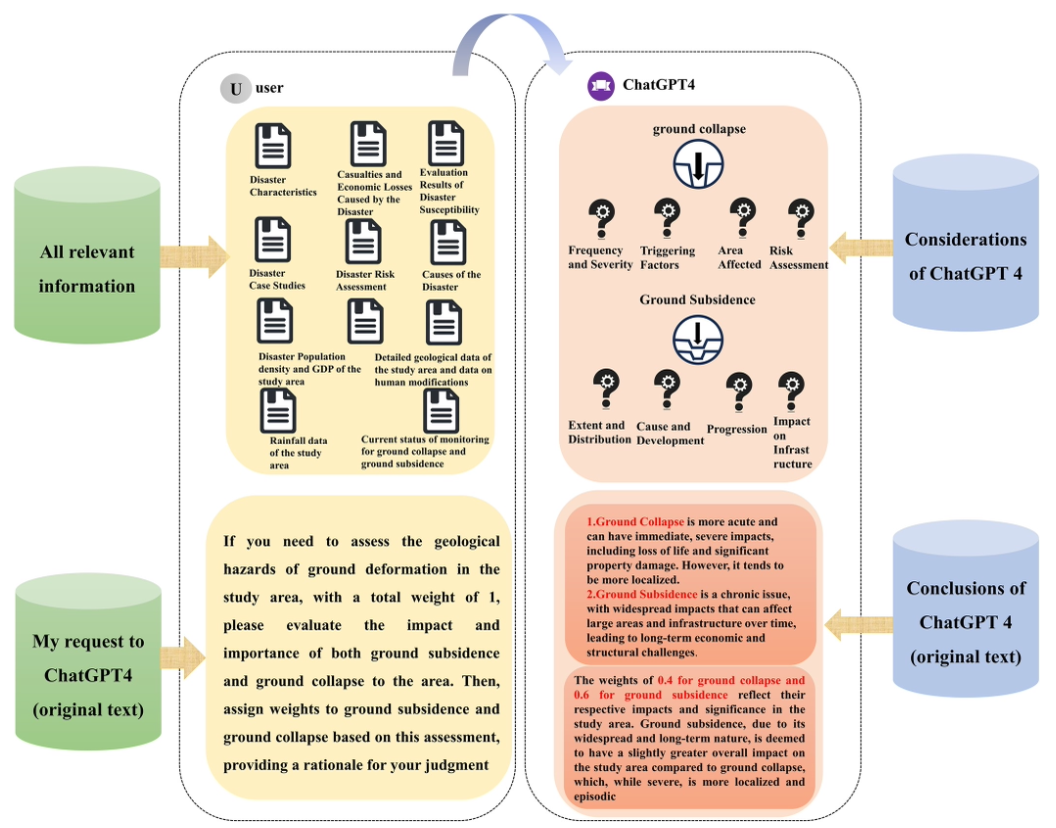
\includegraphics[width=7cm,height=4.5cm]{images/llm}
    \end{column}
\end{columns}

\end{frame}

\begin{frame}{\MakeUppercase{Data authors used}}

\begin{table}[h]
\centering
\begin{tabular}{|l|c|c|}
\hline
\textbf{Name of Data} & \textbf{Size} & \textbf{Accessibility} \\
\hline
Data source files of LLM and code files & 1 long prompt & Public \\
\hline
ArcGIS data & Not shared & Third-party rights \\
\hline
Data processing & 27,898 data points & Used Public \\
\hline
\end{tabular}
\end{table}

\end{frame}

\begin{frame}{\MakeUppercase{What authors shared}}

\begin{itemize}
    \item Prompt for ChatGPT in pdf.
    \item Excel dataset with 27,898 data points for ground subsidence susceptibility assessment.
    \item Code for training and testing (without train/test split) in docx format.
\end{itemize}

\end{frame}

\begin{frame}{\MakeUppercase{What authors are proud about}}
\begin{itemize}
    \item Integrated data-driven models into urban ground collapse and subsidence evaluation.
    \item Used RF-BP neural network coupling model, achieving a 7\% increase in AUC value.
    \item Employed ChatGPT-4 for weight determination, validated by geological experts.
    \item ChatGPT-4's weights differed by only 3\% from expert judgments.
    \item Conducted comprehensive susceptibility assessment using ChatGPT-4's results.
\end{itemize}
\end{frame}


%\section{Examples}

\begin{frame}{\MakeUppercase{Reproducibility}}

\begin{columns}[c]
    \begin{column}{.6\textwidth}
        \begin{itemize}
            \item It is possible to reproduce results!
            \item Authors did not share train/test split code, but provided a good description, allowing reproduction from the description.
            \item Authors achieved 89\% ROC-AUC score for ground collapse binary classification; I achieved 91\%.
            \item I obtained the same weights for ground collapse versus subsidence (weight ratio of 0.4:0.6).
        \end{itemize}
    \end{column}
    \begin{column}{.4\textwidth}
        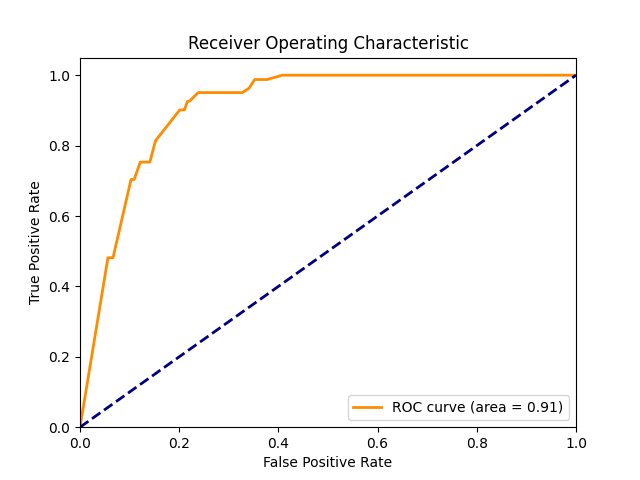
\includegraphics[width=5cm]{output/original_roc_curve}
    \end{column}
\end{columns}

\end{frame}


\begin{frame}{\MakeUppercase{But...}}

Reproducibility \textrightarrow more transparency.

I noted the following issues:

\begin{columns}[c]
    \begin{column}{.5\textwidth}
        1. Factual error on the graphs:
        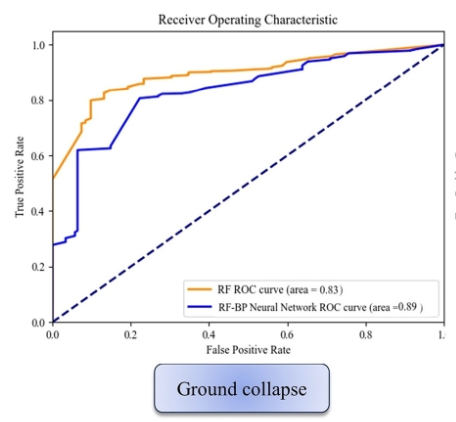
\includegraphics[width=5cm,height=4.5cm]{images/wrong_roc}
    \end{column}
    \begin{column}{.5\textwidth}
        2. Inconsistency between text and graph:
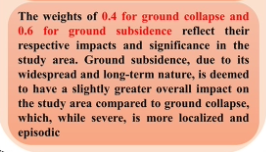
\includegraphics[width=5cm,height=3cm]{images/weights} \\
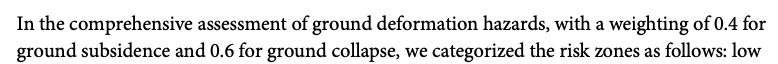
\includegraphics[width=7cm,height=1cm]{images/wrong_weights}
    \end{column}
\end{columns}

\end{frame}


\begin{frame}{\MakeUppercase{Suspicious methodological choices}}

    \begin{itemize}
        \item Strange choice of file formats (docx for Python script, Excel instead of \texttt{.csv}).
        \item Default arguments for Random Forest and Neural Network, no hyperparameter tuning.
        \item Undersampling with Random Forest instead of using class weights.
        \item No data scaling, crucial for Neural Networks with wide value ranges (e.g., 1-178111).
        \item LLM assessment based on a single ChatGPT run, unspecified version and parameters.
    \end{itemize}

\end{frame}



\begin{frame}{\MakeUppercase{My attempts to solve these issues}}

    \begin{itemize}
        \item Added hyperparameter tuning.
        \item Scaled input values.
        \item Changed selection of train values to include all of them and added weight strategy for Random Forest.
        \item Ran multiple experiments with different GPT API models and various temperature values.
    \end{itemize}

\end{frame}

\begin{frame}{\MakeUppercase{Suspicion is growing}}

    \begin{enumerate}
        \item During hyperparameter tuning, I noted that increasing parameters (making the model greedy) leads to better AUC on test data. Usually, greedy models lead to overfitting and failed test results.
        \item LLM models give me 0.4:0.6 weights even on gibberish input.
    \end{enumerate}

\end{frame}


\begin{frame}{\MakeUppercase{More detailed look at data}}

    \textbf{Data check:}
    \begin{itemize}
        \item Noted a lot of similar rows in the data file.
        \item Checked for duplicates and found:
        \begin{itemize}
            \item 27,898 data rows \textrightarrow 625 unique rows.
            \item 296 positive classes \textrightarrow 33 positive examples.
        \end{itemize}
        \item Authors did not mention the problem of duplicated data in the text.
        \item Many duplicates are simultaneously in train (70\% of all rows) and test (30\%).
    \end{itemize}

    \textbf{Conclusion:} To get better results, the model needs to memorize data points.

\end{frame}

\begin{frame}{\MakeUppercase{My alternative aggregation model}}
    \begin{columns}[c]
        \begin{column}{.7\textwidth}
            \begin{itemize}
                \itemsep1em
                \item For this dataset, complex modeling is unnecessary due to extensive data duplication.
                \item A simple dictionary-based approach suffices: match test cases with the training data.
                \item If a test case isn't found in the training data, predict 0, the more frequent class.
            \end{itemize}

            \textbf{Results:} This approach achieves an AUC of 91\%, surpassing the authors' model stack by 2\%.
        \end{column}
        \begin{column}{.3\textwidth}
            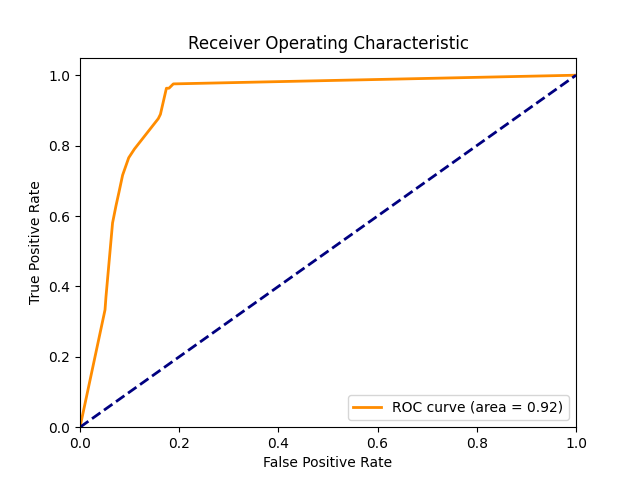
\includegraphics[width=4cm,height=4cm]{output/fake_model_roc_curve}
        \end{column}
    \end{columns}
\end{frame}


\begin{frame}{\MakeUppercase{How results looks like if we do this study correctly}}

\begin{columns}[c]
    \begin{column}{.5\textwidth}
        We won't sell it! Or maybe...
    \end{column}
    \begin{column}{.5\textwidth}
        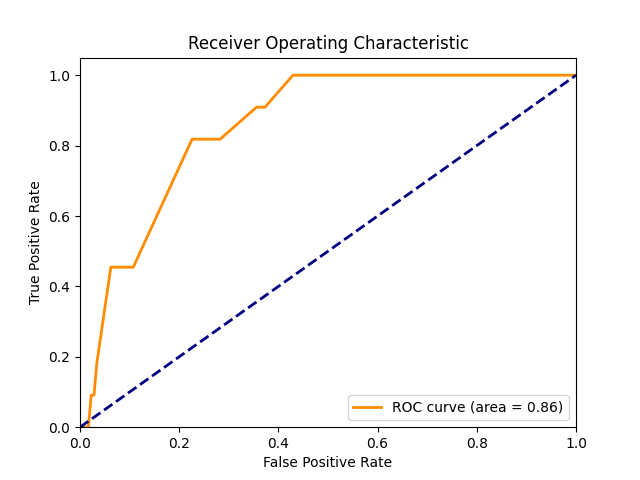
\includegraphics[width=4.5cm,height=4.5cm]{output/alternative_roc_curve}
    \end{column}
\end{columns}

\end{frame}


\begin{frame}{\MakeUppercase{Comparison of different models}}
\begin{columns}[c]
    \begin{column}{.5\textwidth}
        Probably with more time for hyperparameter tuning it's possible to reach the level of broken models.
    \end{column}
    \begin{column}{.5\textwidth}
        \includegraphics[width=4.5cm,height=4.5cm]{output/roc_curve_comparison}
    \end{column}
\end{columns}

\end{frame}


\begin{frame}{\MakeUppercase{LLM runs}}

    Weight 0.4 for Ground Collapse is rather outlier.

    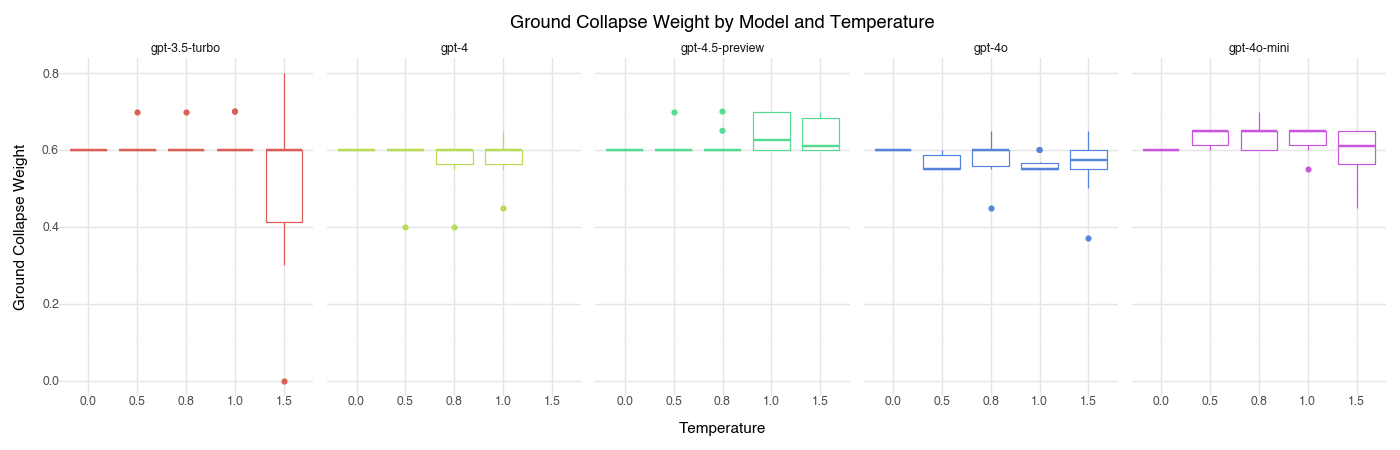
\includegraphics[width=14cm,height=4.5cm]{output/llm_ground_collapse_plot}

\end{frame}

\begin{frame}{\MakeUppercase{LLM runs}}

    Weight 0.4 for Ground Collapse is rather outlier.

    \begin{tabular}{lrrrrrrrr}
\toprule
model & \multicolumn{4}{r}{ground_collapse} & \multicolumn{4}{r}{ground_subsidence} \\
 & mean & std & min & max & mean & std & min & max \\
\midrule
gpt-3.5-turbo & 0.59 & 0.13 & 0.00 & 0.80 & 0.41 & 0.13 & 0.20 & 1.00 \\
gpt-4 & 0.58 & 0.06 & 0.40 & 0.65 & 0.42 & 0.06 & 0.35 & 0.60 \\
gpt-4.5-preview & 0.63 & 0.04 & 0.60 & 0.70 & 0.37 & 0.04 & 0.30 & 0.40 \\
gpt-4o & 0.57 & 0.05 & 0.37 & 0.65 & 0.43 & 0.05 & 0.35 & 0.63 \\
gpt-4o-mini & 0.62 & 0.04 & 0.45 & 0.70 & 0.38 & 0.04 & 0.30 & 0.55 \\
\bottomrule
\end{tabular}


\end{frame}


\begin{frame}{\MakeUppercase{Concluding Thoughts}}

    \begin{itemize}
        \item The quality of reviewers' work in 1Q journals seems lacking; they had ample opportunities to detect these issues but did not.
        \item The study is reproducible, but the practices of sharing code and data could be improved.
    \end{itemize}

\end{frame}



\begin{frame}{\MakeUppercase{Reproducibility of This Reproduction}}

    \begin{itemize}
        \itemsep1em
        \item GitHub repository with data, code for the study and analysis, presentation, and visualizations: \\ \href{https://github.com/RomanKyrychenko/groud_collapse}{\texttt{https://github.com/RomanKyrychenko/groud\_collapse}}
        \item Docker image: \\ \href{https://github.com/RomanKyrychenko/groud_collapse/blob/master/Dockerfile}{\texttt{https://github.com/RomanKyrychenko/groud\_collapse/blob/master/Dockerfile}}
    \end{itemize}

\end{frame}


\end{document}